\chapter{Learning}

Both Machine and Human Learning

\section{Parse and Compile}
TO much time we believe beauty and smartness is in the concise way.

That's only because it's easy to parse, use less data, less to compute, less to distinguish, the beauty is the lazyness, the beauty is the thrift on the limited resource we save for living. Thinking is so demanding and dangerous, pursue beauty, pursue a easier parser.

\subsection{Hardness of Distinguishability}
The strength of neuron connections is for event causation, not features.
The features are how distinguishable a representation can be.
\subsection{Local Environment}
\subsection{Change of Representation}
We can display a line as following ways:

\[ y = x \]

\[ \theta = \dfrac{\pi}{4} \]

\[ \begin{cases}
x = t \\
y = t
\end{cases} \]

\begin{figure}
  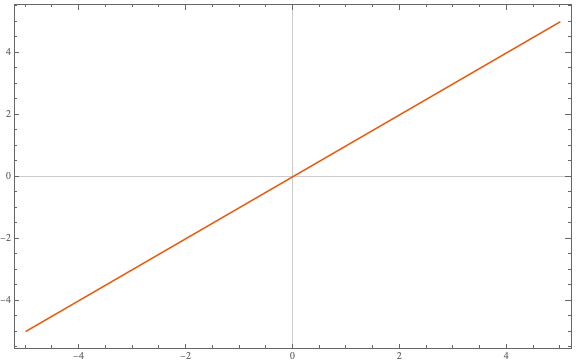
\includegraphics[width=\linewidth]{img/y=x.png}
  \label{fig:y=x}
\end{figure}




\section{Correlation and Fitting}

\section{Causation and Inference}

\section{Mapping and Modeling}

People without sufficient training tend to use a simplified model for the world.

The if $f(a) = positive_result$, people not only believe $f(A) = positive_result$, but also $f(B) = positive_result$. This reduction is so bad that people always blame for the wrong direction. But that also gives engineers a harder problem to solve, you have to solve an over-kill product.


\section{Graph and Linking}

\section{Smartness of a Human Learner}

Rule One: there are distribution of the intelligence. So there are smart children and not so smart kids.

Rule Two: education can change the intelligence but training, not sure how much it can modify. But a humanbeing without any education is hardly able to adapt the modern society.

education change and improve the intelligence. Like software patches to solve hardware deficts.

Rule There: A better designed educational resources will lower the threshold for students so to make knowledge kinds of more accessable.

\subsection{Short-Term Memory}

\subsection{Long-Term Memory}

In my experience, long term memory is the largest obstacle for students to overcome in terms of low level techniques.

It seems like not all brains are good at memorizing stuffs, and I am not sure about the evolutionary benefits of forgetting newly gained knowledge, given so much space to store the information.

\subsection{Sensitivity for Feature Extraction}

Everyone is a pattern recognizor for sure, and that's what separates us from machines.

\subsection{Autocorrection for Flawed Information}

Overcome ambiguity, come up with some patterns to cover the gaps.

Easy to spot on when you crack the source codes. You have to try to guess the meaning of a fragment of codes.

Energy cost is high.

Mapping relating fitting memorizing the facts.

Mapping is the easist. Then is relating.

\subsection{Intensity of Learning Desire}

The desire is generated when problem is at hand, this is my personal experience, I don't know the meaning of learning several subjects. The reason I take courses is because I have to to get my degree, while when I start to solve the real world problem I started to understand that the knowledge and the skill that I learn is to let myself be able to solve the real world problems to let my desire or imagination becomes to reality.

With high motivation, learners are able to tolerant more computational pains.

Also we need to have more learning abilities, which includes how to take notes.

\chapter{Problems}

% introduction
\section{Problems}

To define a problem is defining a class at the same time.

To understand a problem is to know how to check whether one solution is correct or not.
\subsection{Verifying versus Searching}


% types of problems
\section{Types of Problems}
\subsection{Computational Problems}
\subsection{Learning Problems}
\subsection{Generic Problems}

% definition and properties of techniques
\section{Techniques}
The Classification of Techniques is a core concept in daily life.
\begin{figure}
  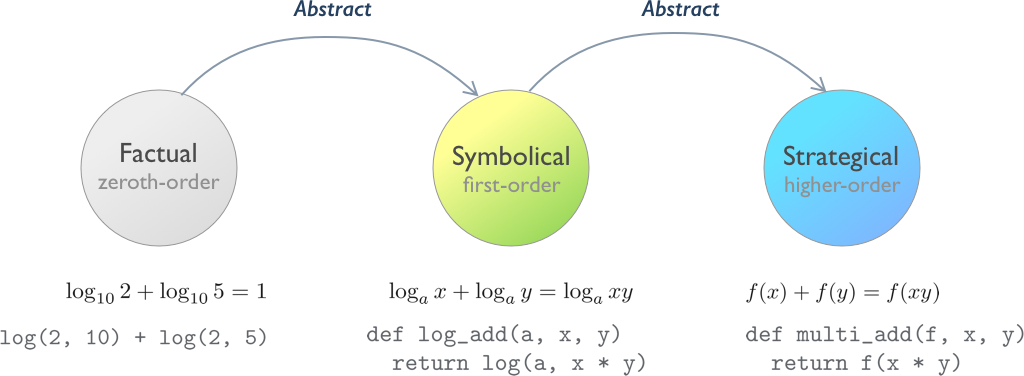
\includegraphics[width=\linewidth]{img/abstract-levels.png}
  \caption{Abstraction Levels}
  \label{fig:abstract-levels}
\end{figure}
\subsection{Robustness of Techniques}
\subsection{Frequency of Usage}
\subsection{Ad-Hoc versus Generic}
One phenominon that I experience a lot is the way people don't distinguish the difference between a ad-hoc technique and a generic technique. When a teacher or a guy present a way to solve a specific problem, few people will appreciate the robustness of this technique, that how well can you transfer your ability on this learning to another situations. But because of their inability to distinguish hardness and robustness, that leads to a dangerous place, that you have to learn too much techniques to cope with every problems, but you don't have enough time for learning these. And the teacher may think by doing an ad-hoc problem will lead to a better understanding for a more generic solving ability, which is vague. You don't learn too much on ad-hoc problems. You only know how to solve it in a nearby situations. The overall hint on a more generic solving strategies are often weak to recognize.

People don't know how to appreciate the robustness of techniques. Only can they find the dramatic changes of events. Even you simply press the button, you believe the underlining changes belongs to your smartness, well the main reason is the engineering behind the scene to smooth the user experience.
\subsection{Intensity of Signal}
\subsection{Trainability of Techniques}
Both the solving radius and the applicability.

% types of techniques
\section{Types of Techniques}
\subsection{Factual Techniques}
\subsection{Algorithmic Techniques}
\subsection{Strategic Techniques}
\subsection{Generic Techniques}
\subsection{Expansion Techniques}


\chapter{Problems}

% introduction
\section{Problems}

To define a problem is defining a class at the same time.

To understand a problem is to know how to check whether one solution is correct or not.
\subsection{Verifying versus Searching}


% types of problems
\section{Types of Problems}
\subsection{Computational Problems}
\subsection{Learning Problems}
\subsection{Generic Problems}

% definition and properties of techniques
\section{Techniques}
The Classification of Techniques is a core concept in daily life.
\begin{figure}
  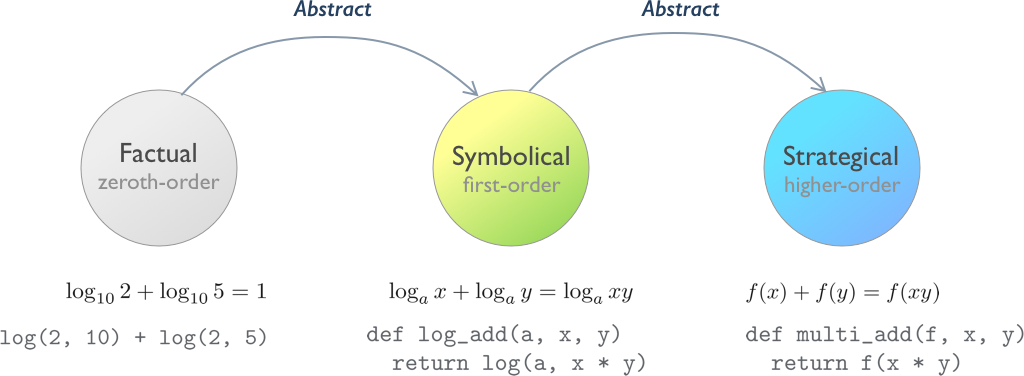
\includegraphics[width=\linewidth]{img/abstract-levels.png}
  \caption{Abstraction Levels}
  \label{fig:abstract-levels}
\end{figure}
\subsection{Robustness of Techniques}
\subsection{Frequency of Usage}
\subsection{Ad-Hoc versus Generic}
One phenominon that I experience a lot is the way people don't distinguish the difference between a ad-hoc technique and a generic technique. When a teacher or a guy present a way to solve a specific problem, few people will appreciate the robustness of this technique, that how well can you transfer your ability on this learning to another situations. But because of their inability to distinguish hardness and robustness, that leads to a dangerous place, that you have to learn too much techniques to cope with every problems, but you don't have enough time for learning these. And the teacher may think by doing an ad-hoc problem will lead to a better understanding for a more generic solving ability, which is vague. You don't learn too much on ad-hoc problems. You only know how to solve it in a nearby situations. The overall hint on a more generic solving strategies are often weak to recognize.

People don't know how to appreciate the robustness of techniques. Only can they find the dramatic changes of events. Even you simply press the button, you believe the underlining changes belongs to your smartness, well the main reason is the engineering behind the scene to smooth the user experience.
\subsection{Intensity of Signal}
\subsection{Trainability of Techniques}
Both the solving radius and the applicability.

% types of techniques
\section{Types of Techniques}
\subsection{Factual Techniques}
\subsection{Algorithmic Techniques}
\subsection{Strategic Techniques}
\subsection{Generic Techniques}
\subsection{Expansion Techniques}


stages of learning:

know about it. follow the procedure. independently solve it.

independently enumerate examples for class level concept.

remember detailed procedures, smooth solving it. internalize it.

recognize and combinate other knowledges under new circumstances.

explore the vicinities of the knowledge

remember more shortcuts (chunks), deep and wide explorations.
